\renewcommand{\chaptername}{\scshape Partie}
\chapter{\normalfont \scshape Effet Schlieren}
\section{Principe du dispositif}
L'air est un fluide transparent, il possède un indice de réfraction qui suit une évolution linéaire par rapport à la densité :
\begin{align}
	n = 1\,+\,k\,\rho
\end{align}
où $\mathnormal{n}$ est l'indice de réfraction du fluide, $\mathnormal{\rho}$ sa densité et $\mathnormal{k}$ une constante appelée constante de Gladstone-Dale~\ref{ref:harvardedu}. Si $\mathnormal{n_i}$ et $\mathnormal{n_r}$ sont respectivement les indices de réfraction des rayons incident et réfléchi, $\mathnormal{\theta_i}$ l'angle d'incidence et $\mathnormal{\theta_r}$ l'angle de réfraction, on peut écrire la loi de Snell-Descartes :
\begin{align}
	n_i\times\,sin(\theta_i) = n_r\times\,sin(\theta_r) 
\end{align}
En faisant varier de manière non uniforme la température ou la pression de l'air, on fait apparaître des gradients de densité, ce qui fait que l'indice de réfraction ne varie pas de la même façon partout dans le fluide. Par conséquent, les rayons lumineux sont déviés, ce qui permet d'observer l'effet Schlieren. Le montage optique peut être réalisé avec un miroir sphérique ou avec deux lentilles convergentes.
\subsection{Dispositif avec miroir sphérique}
\begin{figure}[H]
	\centering
	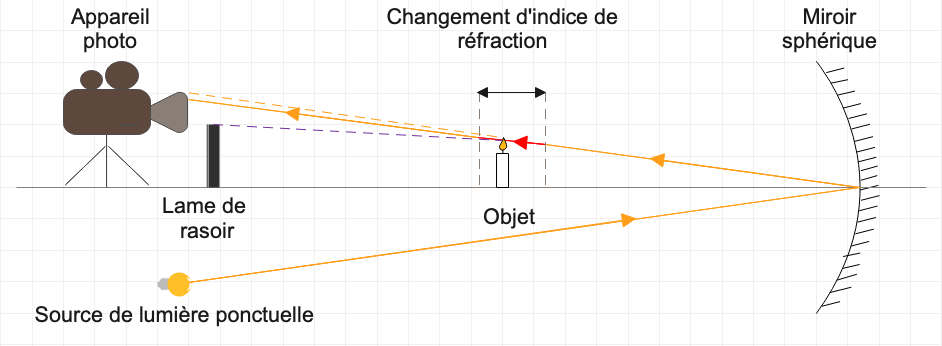
\includegraphics[scale = 0.4]{figures/schlieren_miroir.png}
	\caption{\small{\textit{Schéma du dispositif de Schlieren avec miroir sphérique}}}
	\label{fig:schlieren_miroir}
\end{figure}
Ce dispositif consiste en un miroir sphérique éclairé par une source ponctuelle ; un écran ou une caméra est placé à côté de cette dernière, toujours à une distance égale à deux fois la distance focale du miroir, pour capturer les rayons lumineux réfléchis. Or l’objet à observer est placé en face du miroir, créant une perturbation dans l’air. Certains rayons sont alors déviés, puis coupés par une lame de rasoir qui agit en tant que filtre. On observe ainsi des tâches plus ou moins sombres correspondant à la forme de la perturbation~\ref{ref:harvardedu}.
\subsection{Dispositif avec lentilles convergentes}
\begin{figure}[H]
	\centering
	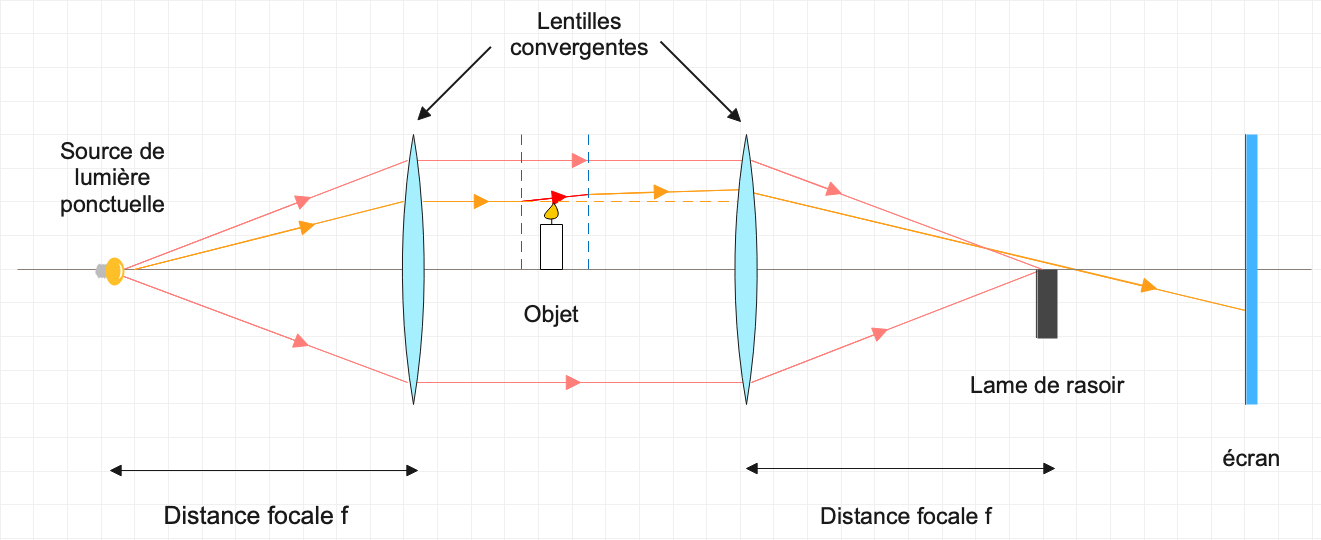
\includegraphics[scale = 0.3]{figures/schlieren_lentilles.png}
	\caption{\small{\textit{Schéma du dispositif de Schlieren avec lentilles convergentes}}}
	\label{fig:schlieren_lentilles}
\end{figure}
Ce système est constitué d'une source de lumière ponctuelle, d'une lame de rasoir, d'un écran et de deux lentilles convergentes faisant office de lentille de Fresnel. On positionne la source ponctuelle au point focal objet de l'une des lentilles afin d'obtenir un faisceau de rayons parallèles, et on se sert de l'autre lentille pour faire converger le faisceau, créant ainsi un système afocal. En plaçant la lame de rasoir au point focal image de la deuxième lentille, on élimine les rayons parallèles au faisceau, ce qui permet d'observer les rayons déviés par effet Schlieren sur l'écran.
\\
\\
Le but de cette première partie est donc de réussir à observer l'influence des gradients de densité sur l'air grâce à l'un des dispositifs énoncés précédemment.
\section{Protocole et organisation}
\subsection{Cahier des charges}
Une fois l'objectif défini, la mise en place d'un plan d'organisation s'est avérée judicieuse pour avancer dans le projet. Pour ce faire, le diagramme de GANTT de la figure~\ref{fig:gantt_schlieren} a été établi :
\begin{figure}[H]
	\centering
	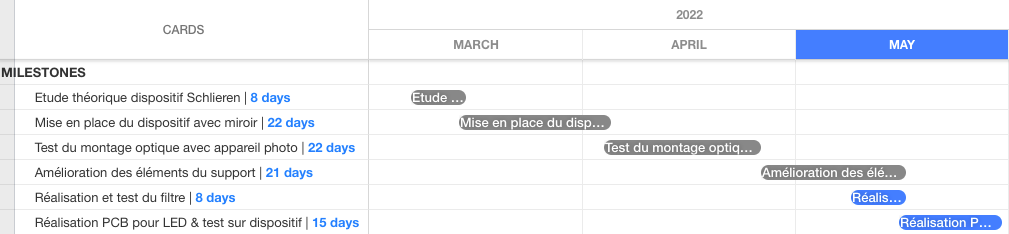
\includegraphics[scale = 0.43]{figures/gantt_schlieren.png}
	\caption{\small{\textit{Diagramme de GANTT prévu pour le montage optique}}}
	\label{fig:gantt_schlieren}
\end{figure}
Par ailleurs, parmi les sept membres du groupe, quatre ont été chargés de mettre en place le système optique, un rôle a été attribué à chacun des membres :
\begin{table}[H]
	\centering
	\setlength{\tabcolsep}{15pt}
	\begin{tabular}{|l l l l|}
		\hline
		\vtop{\hbox{\strut \small\textbf{Responsable}}\hbox{\strut \small\textbf{effet Schlieren}}}&\vtop{\hbox{\strut \small\textbf{Responsable}}\hbox{\strut \small\textbf{communication}}}&\vtop{\hbox{\strut \small\textbf{Responsable}}\hbox{\strut \small\textbf{technique}}}&\vtop{\hbox{\strut \small\textbf{Responsable}}\hbox{\strut \small\textbf{planning}}}\\
		\hline
		\vtop{\hbox{\strut \small{Yvonne}}\hbox{\strut \small{SAUTRIOT}}}&\vtop{\hbox{\strut \small{Léo}}\hbox{\strut \small{LAFFAY}}}&\vtop{\hbox{\strut \small{Alexandre}}\hbox{\strut \small{OCKIER}}}&\vtop{\hbox{\strut \small{Nada}}\hbox{\strut \small{KOUDDANE}}}\\
		\hline
	\end{tabular}
	\caption{\small\textit{Membres et tâches attribuées (dispositif à imagerie Schlieren)}}
	\label{fig:gestion_schlieren}
\end{table}
\subsection{Mise en place des montages optiques}
\subsubsection{\normalfont{\textsc{Montage avec miroir sphérique}}}
Pour ce montage, le matériel suivant a été utilisé :
\begin{itemize}
	\item Un miroir sphérique : \textbf{ø 86 mm}, distance focale : \textbf{520 mm};
	\item Une lame de rasoir;
	\item Une source lumineuse : lampe disponible en salle de TP ou flash de téléphone portable;
	\item Un appareil photo.
\end{itemize}
\subsubsection{\normalfont{\textsc{Montage avec lentilles convergentes}}}
Le système optique avec lentilles convergentes a été constitué à partir des éléments suivants :
\begin{itemize}
	\item Deux lentilles convergentes de distance focale \textbf{50 mm};
	\item Une troisième lentille de distance focale \textbf{35 mm} pour transformer la source lumineuse en une source ponctuelle; 
	\item Une lame de rasoir;
	\item Une source lumineuse : le flash d'un téléphone portable;
	\item Un écran.
\end{itemize}
\subsection{Améliorations des montages}
\begin{figure}[H]
	\centering
	\begin{subfigure}[t]{0.49\textwidth}
		\centering
		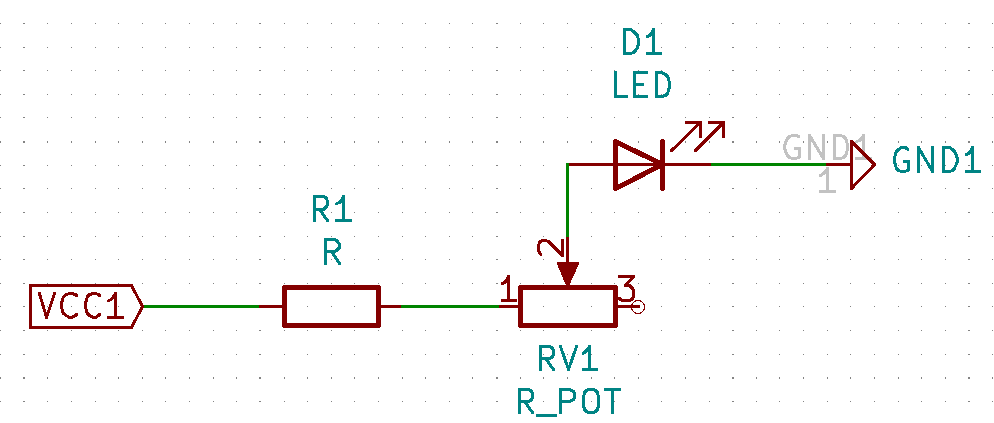
\includegraphics[scale=0.2]{figures/schema_kicad.png}
		\caption{\small{\textit{Schéma Kicad de la LED}}}
		\label{fig:led_kicad}
	\end{subfigure}%
	\begin{subfigure}[t]{0.49\textwidth}
		\centering
		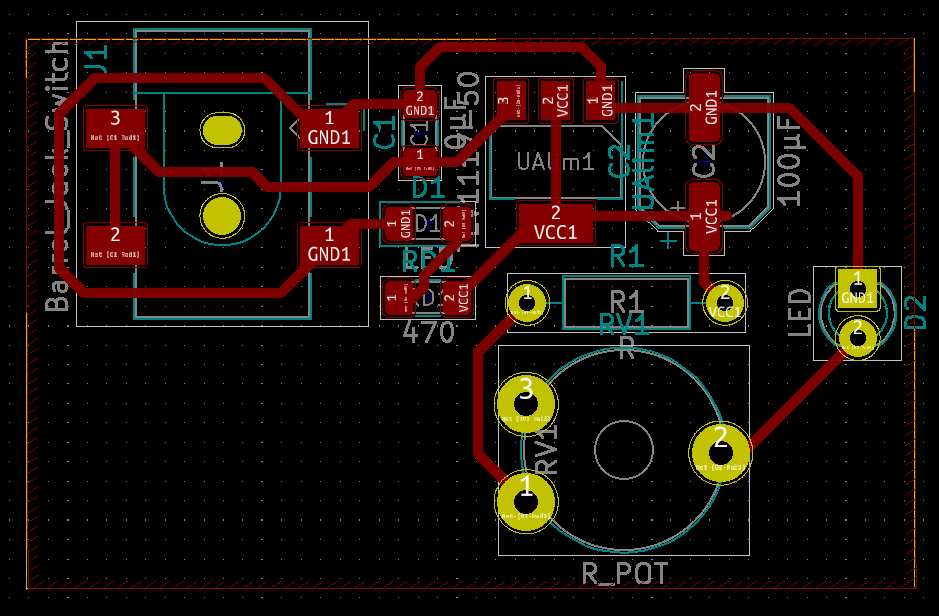
\includegraphics[scale=0.2]{figures/schema_pcb.png}
		\caption{\small{\textit{Schéma de la carte PCB}}}
		\label{fig:led_pcb}
	\end{subfigure}
	\caption{\small{\textit{Schéma du schéma et de la PCB réalisés pour la LED}}}
	\label{fig:led}
\end{figure}
\section{Observations et conclusion}
\subsection{Description des résultats}
\subsection{Interprétation}
\subsection{Conclusion partielle}